%% 
%% Supplementary Material for "Rethinking Decoder Redundancy in Efficient 3D Medical Image Segmentation: A Characterization Study"
%%

\documentclass[final,5p,times,twocolumn]{elsarticle}

\usepackage{amssymb}
\usepackage{amsmath}
\usepackage{graphicx}
\usepackage{booktabs}
\usepackage{multirow}
\usepackage{hyperref}

%% Configure Supplementary Figure / Table numbering (Figure S1, S2...)
\renewcommand{\thefigure}{S\arabic{figure}}
\renewcommand{\thetable}{S\arabic{table}}
\setcounter{figure}{0}
\setcounter{table}{0}

\journal{Computerized Medical Imaging and Graphics}

\begin{document}

\begin{frontmatter}

\title{Supplementary Material: Rethinking Decoder Redundancy in Efficient 3D Medical Image Segmentation: A Characterization Study}

\author[inst1]{Author One\corref{cor1}}
\ead{author1@institute.edu}
\author[inst2]{Author Two}
\author[inst1]{Author Three}

\cortext[cor1]{Corresponding author}

\affiliation[inst1]{organization={Department Name, University Name},
            addressline={Address Line}, 
            city={City Name},
            postcode={00000}, 
            state={State},
            country={Country}}

\affiliation[inst2]{organization={Another Department, Another University},
            addressline={Address Line}, 
            city={City Name},
            postcode={00000}, 
            state={State},
            country={Country}}

\end{frontmatter}

\section*{Supplementary Qualitative Visualizations}

This document provides supplementary qualitative visualizations for SwinUNETR and MedNeXt-M-K3 backbones, complementing the 3D UX-Net qualitative motivation example in Figure 1 of the main manuscript.

\begin{figure*}[htbp]
\centering

\includegraphics[width=0.9\textwidth]{figures/obs-swin-concat/figure1_motivation.png}
\caption{Supplementary Figure S1: Qualitative motivation visualization for SwinUNETR ($E_0$ vs. $E_1$) on BTCV CT multi-organ segmentation. Voxel-level prediction flips (positive corrections and negative degradations) are tightly localized to high-entropy organ boundaries.}
\label{fig:supp_swin}
\end{figure*}

\begin{figure*}[htbp]
\centering
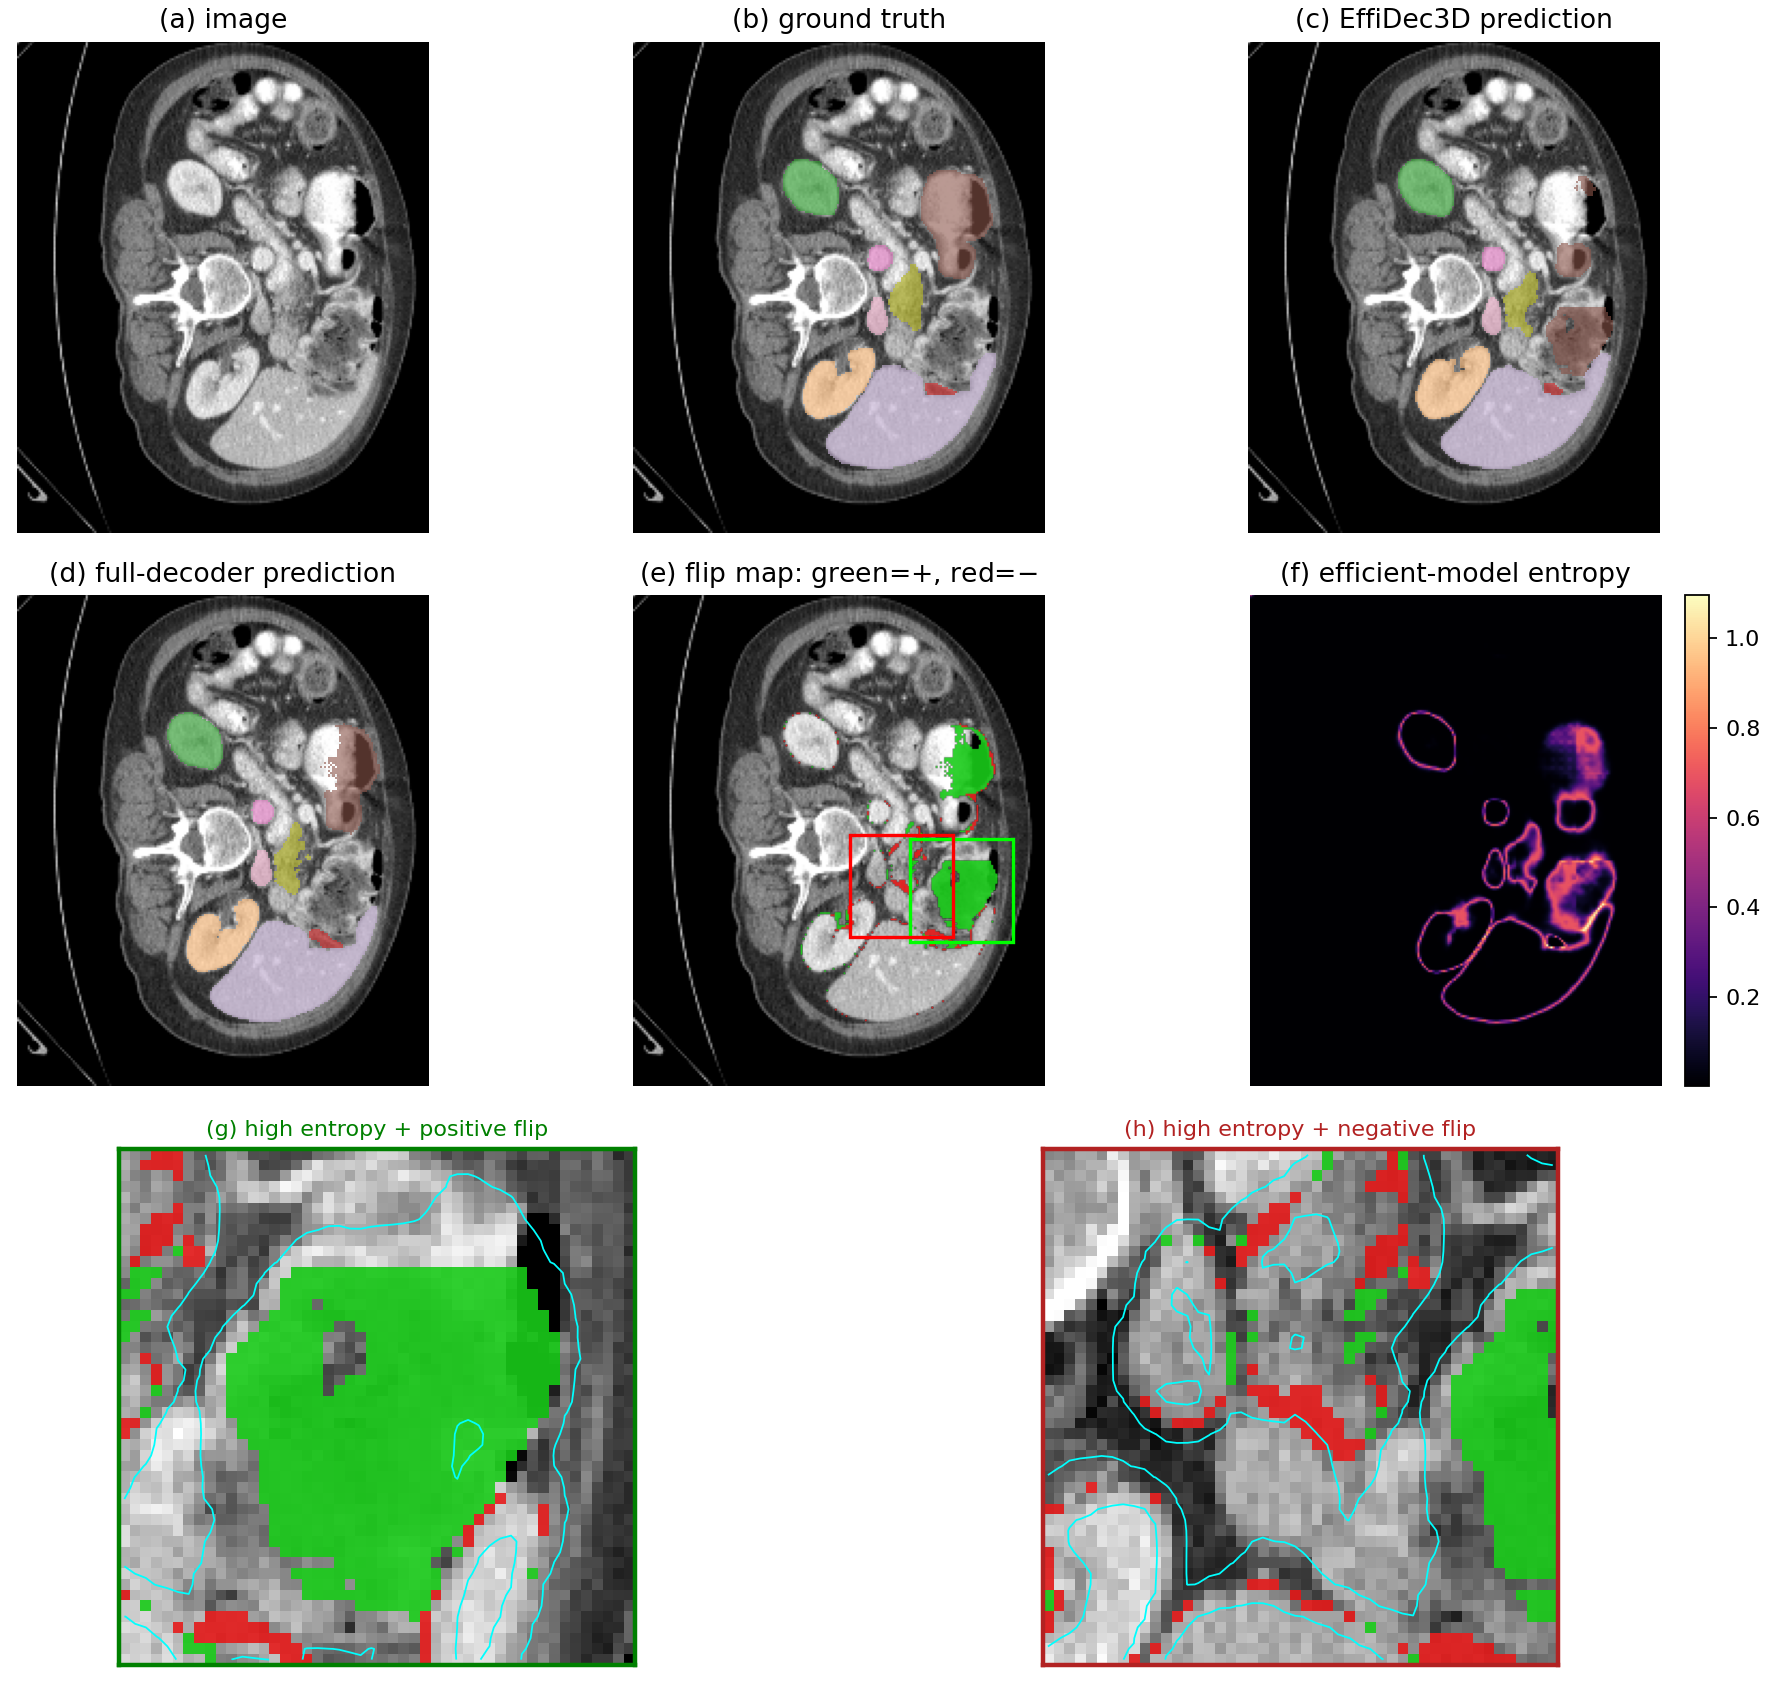
\includegraphics[width=0.9\textwidth]{figures/obs-mednext/figure1_motivation.png}
\caption{Supplementary Figure S2: Qualitative motivation visualization for MedNeXt-M-K3 ($E_0$ vs. $E_1$) on BTCV CT multi-organ segmentation. Consistent with 3D UX-Net and SwinUNETR, decoder-induced flips are concentrated within narrow boundary bands.}
\label{fig:supp_mednext}
\end{figure*}

\end{document}
